\documentclass[english]{beamer}
\usepackage[utf8,latin9]{inputenc}
%%\usepackage[latin9]{inputenc}
\usepackage[T1]{fontenc}
\usepackage{babel}

\usepackage{beamerthemesplit}
\usetheme{Warsaw}
\beamertemplatetransparentcovered

\title{2 years of Londiste}
\author{Dimitri Fontaine}
\date{May, 21 2010}

\begin{document}

\frame{\titlepage}

\section*{Agenda}
\frame{
  \frametitle{Content}
  \tableofcontents[pausesections]
}

\section{Hi-Media Activities}
\frame{

 Online multimedia services: 

 \begin{itemize}
   \item Electronic payment

     \textit{8 millions of transactions, monthly, under constant growth}

   \item Advertising

     \textit{4 billions pages seen, monthly, up to 4000tps}

   \item Interactive Call Services

     \textit{4 millons calls, that's 200 000 hours, monthly}

  \end{itemize}
}

\section{Free Software \& Open Source Toolset}

\frame{
  \frametitle{Open Source Tools}

  We're basically using only Open Source Software in production.

  \begin{itemize}
   \item Apache, haproxy, Nginx
   \item PHP, some tools are in python
   \item Linux, debian, FreeBSD
   \item PostgreSQL
  \end{itemize}
}

\begin{frame}[fragile]
  \frametitle{Monitoring}
  \begin{center} We use \textit{Nagios} and \textit{Munin}. \end{center}
  \begin{overprint}
  \onslide<1>
  \begin{center} 
    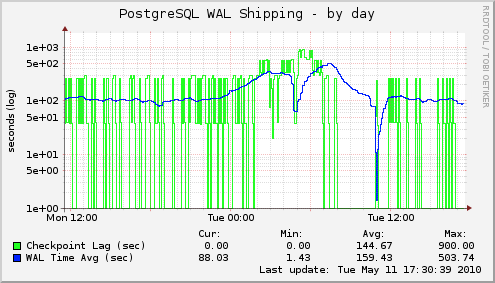
\includegraphics[height=2.0in]{bdd-pg_walmgr-day.png}
  \end{center} 

  \onslide<2>
  \begin{center} 
    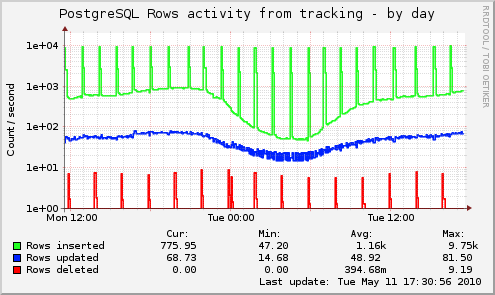
\includegraphics[height=2.0in]{tr1-pg_user_tables_activity_tracking-day.png}
  \end{center} 

  \onslide<3>
  \begin{center} 
    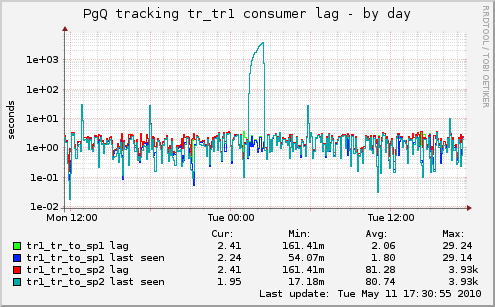
\includegraphics[height=2.0in]{tr1-pg_queue_tracking_tr_tr1-day.png}
  \end{center} 

  \onslide<4>
  \begin{center} 
    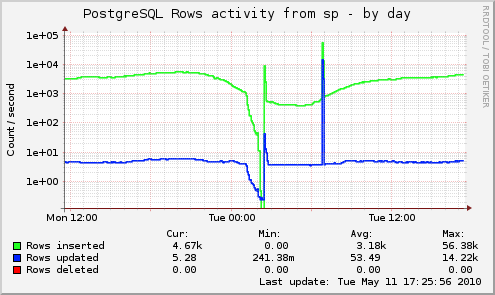
\includegraphics[height=2.0in]{sp2n-pg_user_tables_activity_sp-day.png}
  \end{center} 

  \end{overprint}  
\end{frame}

\frame{
  \frametitle{pgFouine} 

  \texttt{pgFouine} parses and analyses our logs 

\begin{itemize}
    \item<1-> it produces easy to digest \texttt{HTML} reports
    \item<2-> it sends emails with the errors, too
    \item<3-> allows for targetting the optimisation effort
\end{itemize}

}

\subsection{Performances}

\frame{
  \frametitle{Latency is good}

  \begin{itemize}
    \item<1-> About \texttt{6ms} to push an advert
    \item<2-> \texttt{300 tps} in average
    \item<3-> replication lag is setup for averaging at \texttt{3s}
    \item<4-> we switched from another open source solution, we're much better now
  \end{itemize}
}

\subsection{Production Environment}
\frame{
  \frametitle{Production}

  Using from \texttt{8.2} to \texttt{8.4} in production:
	
  \begin{itemize}
    \item<2-> about 50 production databases
    \item<3-> anywhere from some \texttt{MB} to \texttt{1518 GB}
    \item<4-> OLTP (\textit{very low latency})
    \item<5-> OLAP (\textit{bigger volumes, high insert load})
    \item<6-> using distribution packages only
  \end{itemize}
}

\subsection{Human Resources}
\frame{
  \frametitle{I just work there}
  We're 2 DBA with a high specialisation on PostgreSQL. What we do is

  \begin{itemize}
    \item<1-> manage the production 
    \item<2-> participate into development (lots of logic is in the database)
    \item<3-> enhance the tool set, proposing Open Source Software each time
      it makes sense
  \end{itemize}
}

\section{Replication and failover}

\subsection{Different Architectures for different needs}

\frame{
  \frametitle{Centralised management and data federating}

  Include a graphic, talk about it
}

\frame{
  \frametitle{Separating payments and their backoffice}

  Include a graphic, talk about it
}

\frame{
  \frametitle{Modernizing ditributed delivery}

  Include a graphic, talk about it
}

\subsection{Skytools}

\frame{
  \frametitle{Replication, Queuing}

  We use Skype tool suite, which is Open Source

  \begin{definition}
    \alert{\texttt{londiste}} Asynchronous master/slave replication

    \alert{\texttt{PGQ}} Queuing and asynchronous batches, still transactional

    \alert{\texttt{WalMgr}} WAL Shipping (\textit{failover})

    \alert{\texttt{pgbouncer}} connection pooling (\textit{prepared statements!})

    \alert{\texttt{plproxy}} alternative transport mechanism, and RPC solution
  \end{definition}
}

\subsection{Transactional Batch processing}
\frame{
  \frametitle{Using PGQ for batch needs}

  We have all this code in PHP, and we need to process data after the client
  saw the \textt{COMMIT} back. We want to be able to stop them and never
  lose a single transaction, even if system crashes. PostgreSQL level
  reliability. \texttt{PGQ} offers that, for \texttt{python}.

  \linebreak
  \linebreak
  \pause

  \begin{center} \texttt{libphp-pgq} \end{center}
}

\section{Open Source Community}

\subsection{Community \& PgFoundry}

\section{Conclusion}

\subsection{Reliable solution}

\frame{
  \frametitle{Multiple usages of replication}

  We use replication for serving quite different needs

  \begin{itemize}
    \item<2-> Separate different application layers
    \item<3-> Federating logs and offloading their processing
    \item<4-> Managing information on 1 backoffice only, but having network
      glitches tolerant front servers, or cached data if you will
    \item<5-> Materialized views for more than one server
    \item<6-> \textit{Failover} ready
  \end{itemize}
}

\subsection{Any question?}

\frame{
  \frametitle{Any question?}

  \begin{center}
    Now is a pretty good time to ask!
  \end{center}

  \linebreak
  \pause

  %% \begin{center}
  %%   If you want to leave feedback, consider visiting
  %%   \url{http://2009.pgday.eu/feedback}
  %% \end{center}
}


\end{document}


